\chapter{Implementation Details}

Building on the methods described in the previous chapter, this chapter focuses on the practical aspects of our work.
Specifically, it covers the architecture design, evaluation metrics, datasets, and preprocessing steps used in our experiments.

\section{Architecture}\label{sec:architecture}

\begin{wrapfigure}{r}{0.48\textwidth}
    \vspace{-12pt}
    \centering
    
\includegraphics[width=0.48\textwidth]{img/fig_5.1.png}
    \caption{
        Denoised results for both skip connection variants.
        Both images are obtained using SG-DIP\@.
        The ECA-based variant retains more structural details compared to the convolution-based approach.
    }\label{fig:ECA}
\end{wrapfigure}
All architectures in our experiments use a fully-convolutional encoder-decoder network with skip connections, following the U-Net~\cite{U-Net} architecture.
The encoder progressively downsamples the input using strided convolutions, increasing the number of feature channels while reducing spatial resolution.
The decoder then upsamples the feature representations back to the target resolution using bilinear upsampling followed by additional convolutions.
Skip connections are employed between corresponding encoder and decoder layers, bypassing the bottleneck to preserve fine-grained details.
This helps retain spatial information that would otherwise be lost due to downsampling, thereby improving reconstruction quality.
We find that parameterizing these skip connections is crucial for achieving strong denoising performance.
While the original DIP paper employs $1 \times 1$ convolutions in the skip connections, we also explore a variant that replaces these convolutions with ECA blocks.
We find that both variants yield comparable performance in terms of PSNR and SSIM\@; however, ECA blocks often contribute to better preservation of fine details, as shown in Figure~\ref{fig:ECA}.

As in the original DIP paper, Batch Normalization (BN) is applied throughout the network.
Note that for the DIP setting, BN is actually equivalent to Instance Normalization, as the batch size is 1 and there is no difference between training and inference time.
All activation functions used in the network are LeakyReLU~\cite{LeakyReLU}.
LeakyReLU extends ReLU by allowing a small slope for negative values, ensuring non-zero gradients throughout the domain.
Formally, it is defined as
\begin{equation}
    \varphi(x) = \begin{cases}
        x &\text{if}\ x \geq 0\\
        \alpha x &\text{if}\ x < 0,
    \end{cases}
\end{equation}
where $\alpha = 0.2$ in our case.
Unless noted otherwise, all experiments employ the architecture visualized in Figure~\ref{fig:architecture}, implemented using PyTorch~\cite{PyTorch}.
Optimization is performed using the Adam optimizer~\cite{Adam} with a learning rate of 0.01.

\begin{figure}
    \centering
    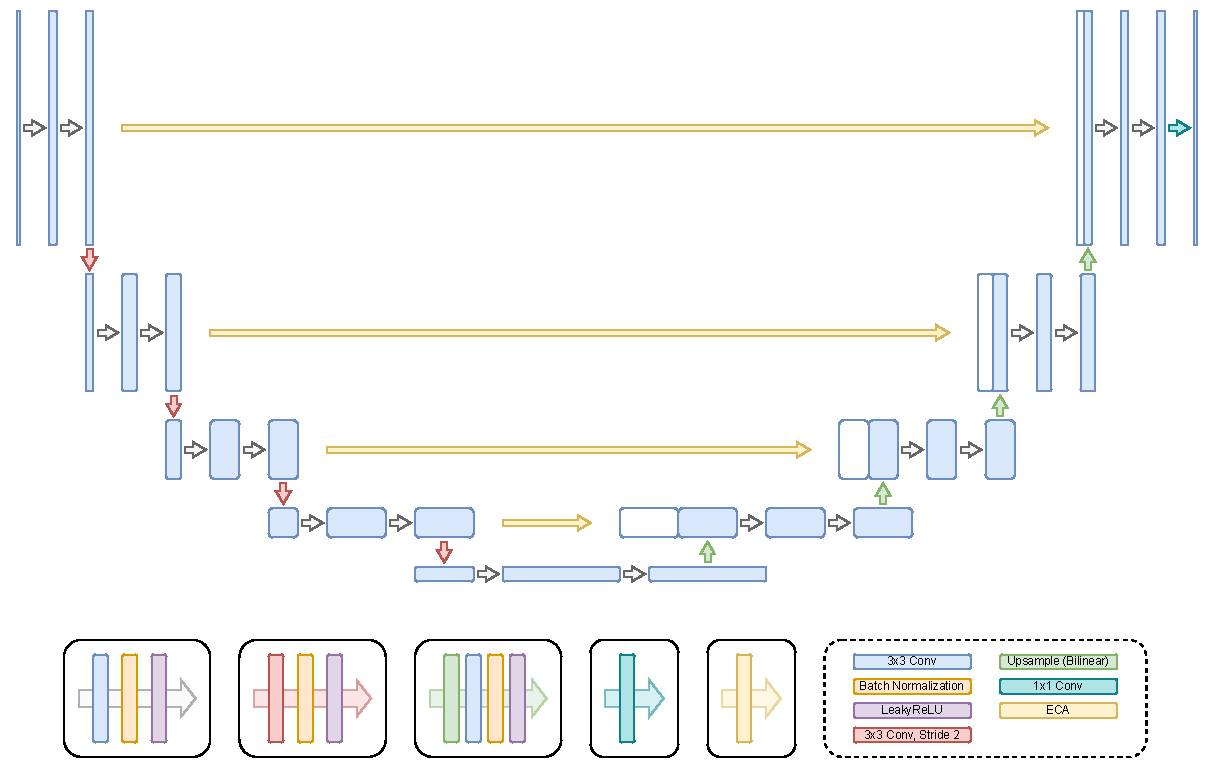
\includegraphics[width=\textwidth]{img/fig_5.2.pdf}
    \caption{
        Architecture used in our experiments.
        Each blue box corresponds to a multi-channel feature map, while white boxes represent copied feature maps, reweighted using ECA\@.
        Different colored arrows denote various operations, detailed in the boxes below (e.g., gray for convolution blocks, red for downsampling blocks, etc.).
        Figure adapted from~\cite{U-Net} and~\cite{DIP}.
    }\label{fig:architecture}
\end{figure}

\newpage

\section{Metrics}

To evaluate and compare the performance of different denoising methods, we rely on two widely used image quality metrics: Peak Signal-to-Noise Ratio (PSNR) and Structural Similarity Index Measure (SSIM).

\subsection{Peak Signal-to-Noise Ratio}

PSNR is a standard metric used to quantify the reconstruction quality of an image by measuring the ratio between the maximum possible pixel intensity and the mean squared error (MSE) between the original and denoised images, $x, \hat{x} \in \R^{W \times H}$.
It is defined as:
\begin{equation}
    \text{PSNR}(x,\hat{x}) = 10 \cdot \log_{10} \left(\frac{x_{\text{max}}^2}{\text{MSE}(x,\hat{x})}\right),
\end{equation}
where $x_{\text{max}}$ is the maximum possible pixel intensity.
For a normalized image, $x_{\text{max}} = 1$, therefore we obtain the simplified definition
\begin{equation}\label{eq:PSNR}
    \text{PSNR}(x,\hat{x}) = 10 \cdot \log_{10} \left(\frac{1}{\text{MSE}}\right) = -10 \cdot \log_{10}(\text{MSE}(x,\hat{x})),
\end{equation}
where the MSE is given by
\begin{equation}\label{eq:MSE}
    \text{MSE}(x,\hat{x}) = \frac{1}{W \cdot H} \sum_{i=1}^{W} \sum_{j=1}^{H} (x_{i,j} - \hat{x}_{i,j})^2.
\end{equation}
For color images with dimensions $3 \times W \times H$, the MSE is additionally computed across the 3 color channels.

A higher PSNR value indicates better image quality, with less distortion introduced by the denoising process.
However, PSNR is a pixel-wise metric that does not account for perceptual quality, therefore we also consider the SSIM\@.

\subsection{Structural Similarity Index Measure}

SSIM~\cite{SSIM} is designed to assess perceptual similarity between images by considering structural information, contrast, and luminance. It is computed as:
\begin{equation}
\text{SSIM}(x, \hat{x}) = \frac{(2\mu_x \mu_{\hat{x}} + c_1)(2\sigma_{x\hat{x}} + c_2)}{(\mu_x^2 + \mu_{\hat{x}}^2 + c_1)(\sigma_x^2 + \sigma_{\hat{x}}^2 + c_2)}
\end{equation}
where $\mu_x$ and $\mu_{\hat{x}}$ are the mean intensities of the original and denoised images, $\sigma_x^2$ and $\sigma_{\hat{x}}^2$ are their variances, and $\sigma_{x\hat{x}}$ is the covariance between them.
The constants $c_1$ and $c_2$ stabilize the division, preventing numerical instabilities when the denominator is close to zero.
SSIM values range from 0 to 1, with higher values indicating better structural similarity.
Unlike PSNR, SSIM is more aligned with human perception, making it a crucial metric for evaluating image denoising performance.

% TODO add local waveform coherence (CC)

\section{Datasets}

This section describes the datasets used in our experiments for both image and distributed acoustic sensing (DAS) data.

\subsection{Image Datasets}

We use three standard image datasets commonly employed for image denoising tasks:
\begin{itemize}
    \item \textbf{Set14}~\cite{Set14}: A small dataset consisting of 14 images, widely used for evaluating image restoration algorithms.
    \item \textbf{CBSD68}~\cite{CBSD68}: A dataset containing 68 natural images from the Berkeley segmentation dataset, commonly used for benchmarking denoising methods.
    \item \textbf{CelebA}~\cite{CelebA}: A large-scale face dataset with over 200,000 images, useful for evaluating denoising performance on human faces.
\end{itemize}

To generate a noisy image $\hat{x}$ from a clean image $x$ at a predefined PSNR level, we add Gaussian noise $n \sim \normal$, where $\sigma^2$ is determined by the desired PSNR\@.
Because the noise is additive, substituting $\hat{x} = x + n$ into Equation~\ref{eq:MSE} simplifies it to
\begin{equation}
    \text{MSE}(x,\hat{x}) = \frac{1}{W \cdot H} \sum_{i=1}^{W} \sum_{j=1}^{H} n_{i,j}^2.
\end{equation}
Since the noise is also zero-mean, we approximate $\sigma^2 \approx \text{MSE}$.
Rewriting Equation~\ref{eq:PSNR} in terms of MSE, we get
\begin{equation}
    \text{MSE}(x,\hat{x}) = 10^{-\frac{\text{PSNR}(x,\hat{x})}{10}}.
\end{equation}
For a given PSNR value, we can therefore obtain a corresponding noisy image as
\begin{equation}
    \hat{x} = x + \sigma\epsilon, \quad \epsilon \sim \unormal,
\end{equation}
where $\sigma = \sqrt{10^{-\frac{\text{PSNR}(x,\hat{x})}{10}}}$.

\subsection{Distributed Acoustic Sensing Datasets}

% TODO add experiment details (see Mattermost)
For denoising DAS data, we use data from two real-world experiments:
\begin{itemize}
    \item \textbf{SISSLE}~\cite{SISSLE}: The South Island Seismology at the Speed of Light Experiment near Haast, New Zealand.
    \item \textbf{FORGE}~\cite{FORGE}: The Frontier Observatory for Research in Geothermal Energy in Utah.
\end{itemize}
Exact sources for the samples used in our experiments can be found in the supplementary material.

% XXX synth data

\section{Preprocessing}

% TODO local normalization channel wise
This section discusses preprocessing steps applied to the input before passing it to DIP-based methods.
For image data, no specific preprocessing is needed.
After generating noisy samples as described in the last section, we simply standardize the inputs to zero mean and unit variance.

For DAS data, however, appropriate preprocessing is crucial for the success of DIP-based methods.
As discussed in Section~\ref{sec:DAS}, noise in DAS measurements often exhibits a grid-like structure, mainly due to erratic and common mode noise.
This structured noise is repetitive and spatially correlated, and therefore inherently easy to learn for a convolutional network, which contradicts a key assumption of DIP --- that meaningful signal is learned faster than noise.
To mitigate this issue, following~\cite{IDF}, we first apply a low-pass filter with a high-cut frequency of 200\,Hz.
To further remove common mode noise, we subtract the time-wise median from the filtered signal.

Another challenge arises due to the large variations in amplitude within DAS measurements.
DIP-based methods, particularly SG-DIP, tend to focus on high-amplitude regions while neglecting lower-amplitude parts.
To address this, we propose using a local normalization approach.
Specifically, we divide the input into overlapping local regions and compute the mean and standard deviation within each window.
Each region is then normalized independently to have zero mean and unit variance:
\begin{equation}
    x'_{i,j} = \frac{x_{i,j} - \mu_{i,j}}{\sigma_{i,j}},
\end{equation}
where $\mu_{i,j}$ and $\sigma_{i,j}$ are the mean and standard deviation computed within a local window centered at $(i,j)$.
In practice, we use a window size of $32 \times 32$.

After DIP-based processing, we rescale the output using the stored local mean and standard deviation to restore the original amplitude relationships.
The different preprocessing steps are visualized in Figure~\ref{fig:preprocessing}.

\begin{figure}
    \centering
    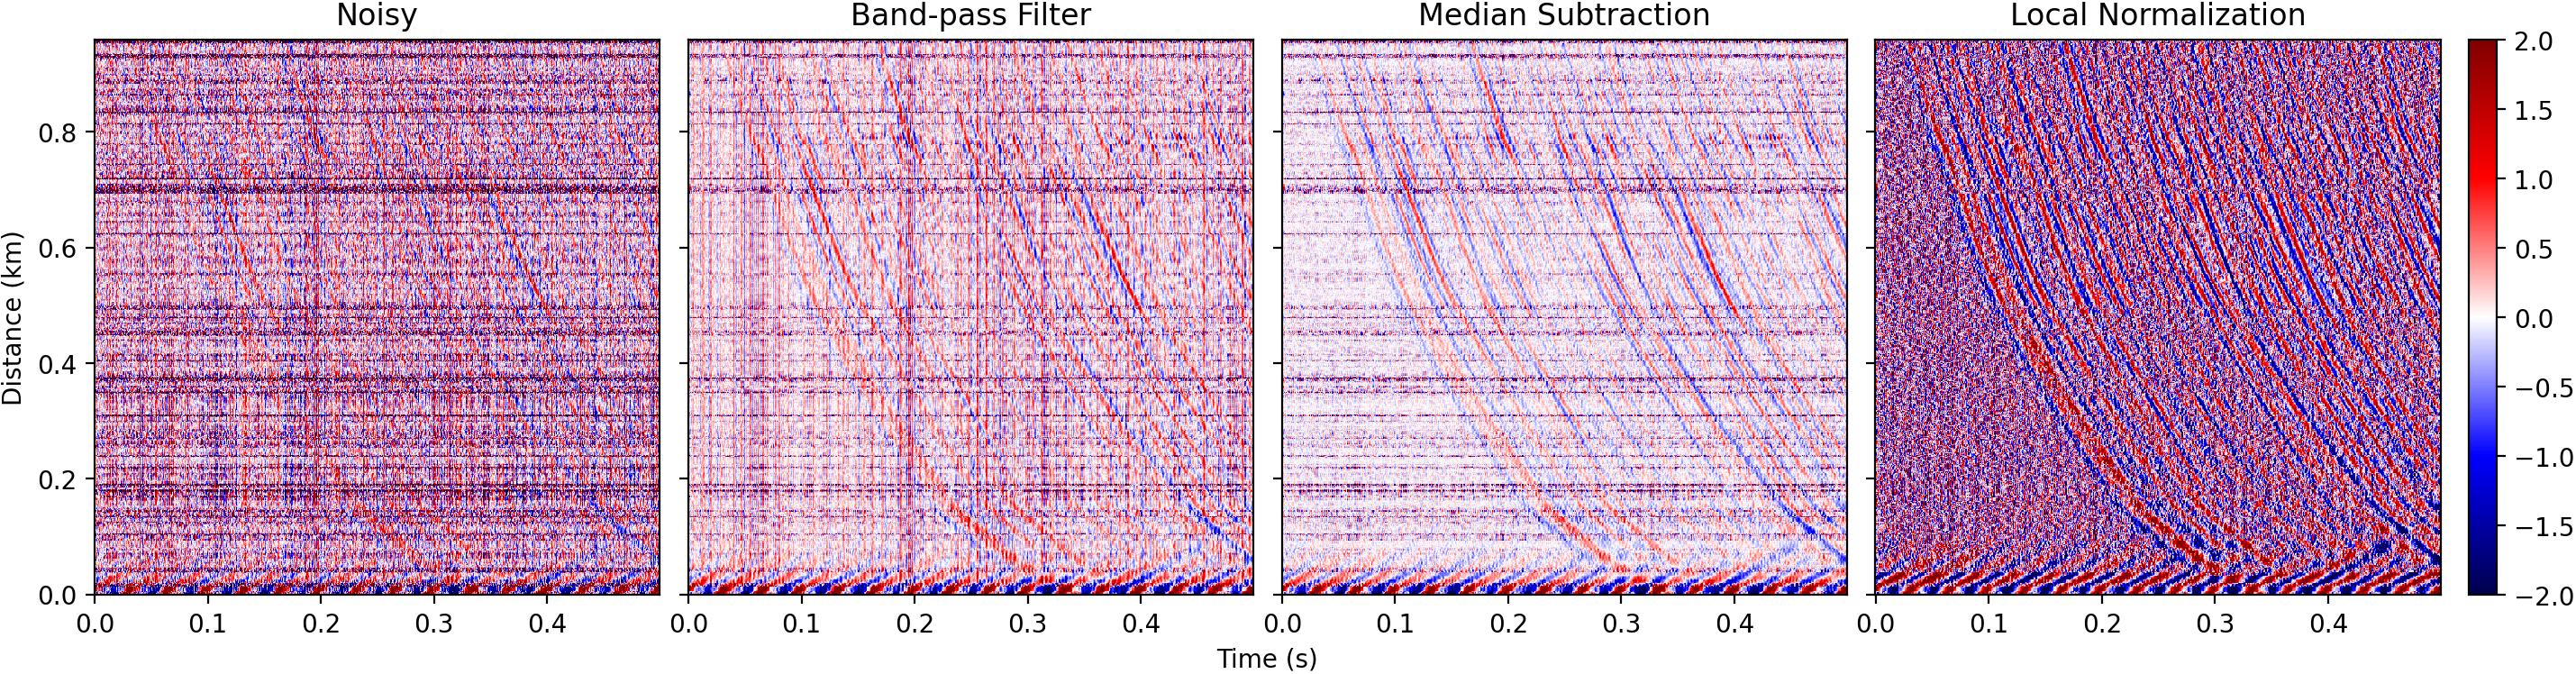
\includegraphics[width=\textwidth]{img/fig_5.3.png}
    \caption{
        Different preprocessing steps.
        The noisy input is first normalized by its standard deviation.
        The following measurements are then obtained by sequentially applying the specified operations.
    }\label{fig:preprocessing}
\end{figure}
